% !TEX root = ../../../main.tex
% 来源：中学数学实验教材·第三册（高中数学）
% 章节：二次函数 / 二次函数
% 原始文件：5.tex，行 30-44
% 类型：tikz
% ---
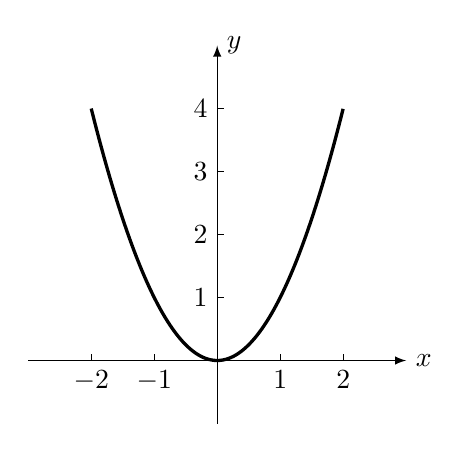
\begin{tikzpicture}[>=latex, scale=.8]
\draw[->](-3,0)--(3,0)node[right]{$x$};
\draw[->](0,-1)--(0,5)node[right]{$y$};
\foreach \x in {-2,-1,1,2}
{
    \draw (\x,0)node[below]{$\x$}--(\x, 0.1);
}
\foreach \x in {1,2,...,4}
{
    \draw (0,\x)node[left]{$\x$}--(.1,\x);
}

\draw[domain=-2:2, samples=100, very thick] plot(\x,{\x*\x});

\end{tikzpicture}
